
\documentclass[journal,12pt,onecolumn,draftclsnofoot]{ieeeconf}  % Comment this line out if you need a4paper

\usepackage{listings}
\usepackage{hyperref}
\usepackage{url}
\usepackage[pdftex]{graphicx}
\usepackage{amsfonts}
\usepackage{subfigure} 
\usepackage{algorithm}
%\usepackage{algorithmic}
\usepackage{amsmath}
\usepackage{bm}
\usepackage{algcompatible}
\usepackage{framed}
\usepackage{balance}

\usepackage{graphics} % for pdf, bitmapped graphics files
\usepackage{caption}
\usepackage{epsfig}
\usepackage{wrapfig}
\usepackage{breqn}

\DeclareMathOperator*{\argmax}{arg\,max}

\pdfminorversion=4

\IEEEoverridecommandlockouts                              % This command is only needed if 
                                                          % you want to use the \thanks command
\overrideIEEEmargins                                      % Needed to meet printer requirements.

\author{Wenbo Xu, Wenwen Zhang, Yichi Zhang}

\title{
	EE 382C: Multicore Computing \protect\\
	\Large \bf Parallel GPU based Algorithms for Image Processing
}

\begin{document}
\maketitle
\thispagestyle{empty}
\pagestyle{empty}


\section{Abstract}
  

\section{Introduction}

\section{Gaussian filter}

\section{Optimization}

\subsection{Pageable vs. Pinned Memory}
Host data allocations are pageable by default, which means can be paged in/out between RAM and disk. However, GPU cannot access data directly from pageable memory, but from pinned memory, which means page-locked. Hence, whenever a data transfer is invoked on pageable memory, the CUDA driver has to allocate a temporary pinned memory array to copy host data and then transfer it to the device. \par
\begin{figure}[h]
	\centering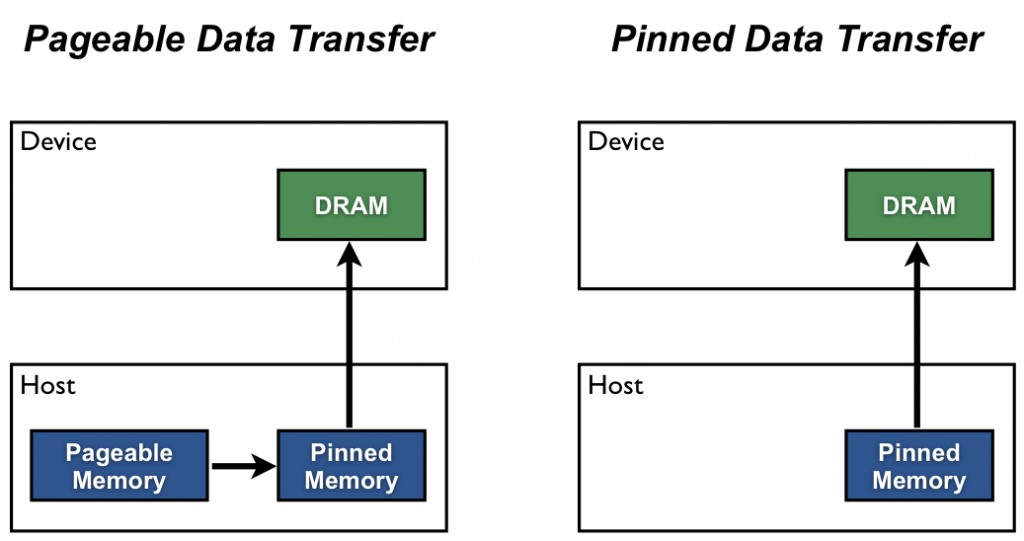
\includegraphics[width=120mm]{pinned.jpg}
	\caption{CUDA data transfer.\cite{Mark}}
	\label{CUDA data transfer.}
\end{figure}
We can avoid the cost of this overhead by using pinned memory for host instead of pageable memory. In this case, we use \textit{cudaMallocHost()} and \textit{cudaFreeHost()}. Compare to the \textit{malloc()} and \textit{free()}, \textit{cudaMallocHost()} and \textit{cudaFreeHost()} are more expensive with additional overheads. Then, the question has been raised about how should we made the tradeoff. According to figure below, pinned memory is faster when the size of data to be transfered is larger than 16MB.  	\cite{Trade_off}\par
\begin{figure}[h]
 	\centering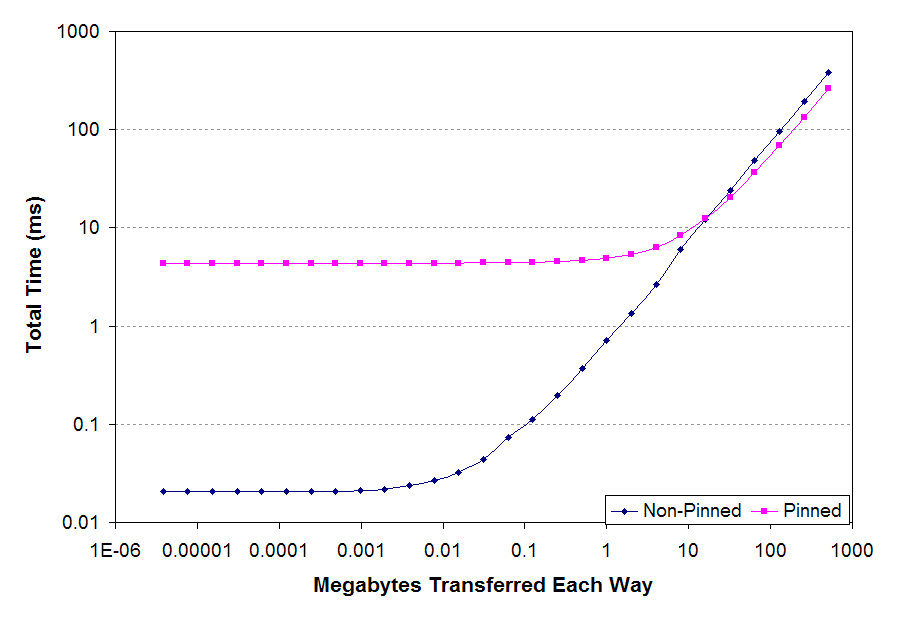
\includegraphics[width=120mm]{pinned_trade_off.png}
 	\caption{Time required to allocate, transfer to the GPU, transfer back to the CPU, and deallocate pinned and non-pinned memory.\cite{Trade_off}}
 	\label{Time required to allocate, transfer to the GPU, transfer back to the CPU, and deallocate pinned and non-pinned memory.}
\end{figure}
This doesn't means we should never use pinned memory when the amount of data to be transfered is less than 16MB. One example is the asynchronous memory copy, \textit{cudaMemcpyAsync()} can be used only with pinned memory. The details of how asynchronous memory copy would be used to improve the efficiency will be discussed in next section.

\subsection{Streams}
A stream is defined as a sequence of operations in that execute in issue-order on the GPU. CUDA operations, which are kernal operations and memory operations, in same streams are ordered and in different streams can overlap. By default, all operations are in default stream. The following code is used to specify which stream the operation is in. \par

\begin{lstlisting}
for (int i = 0; i < nStreams; ++i) {
int offset = i * streamSize;
cudaMemcpyAsync(&d_a[offset], &a[offset], streamBytes,cudaMemcpyHostToDevice, cudaMemcpyHostToDevice, stream[i]);
}
for (int i = 0; i < nStreams; ++i) {
int offset = i * streamSize;
kernel<<<streamSize/blockSize, blockSize, 0, stream[i]>>>(d_a, offset);
}
for (int i = 0; i < nStreams; ++i) {
int offset = i * streamSize;
cudaMemcpyAsync(&a[offset], &d_a[offset], streamBytes,cudaMemcpyDeviceToHost, cudaMemcpyDeviceToHost, stream[i]);
}

\end{lstlisting}

The code shown above is an example of invocation of multiple streams in CUDA. The code is divided into three parts, memory copy form Host to Device, kernel invocation, and memory copy from Device to Host. For memory copies, \textit{cudaMemcpyAsync()} is used. As described in last section, we have to allocate pinned memory using \textit{cudaMallocHost()}. This method place transfer into the stream and returns immediately. It is upto device to schedule streams when the corresponding resources are free. It allows us to put memory transfer operations and kernel operations into the stream the same time and allow them to run concurrently.\cite{Stream} \par
The figure below illustrate the execution time line for three different scenarios. The top time line shows time line without use of streams, which all operations executes in sequential order. The time line in the middle shows the use of streams on hardware has only one copy engine. The performance improvement is significant. The bottom time line shows the time line for hardware has two copy engines. With two copy engines, the HD (Host to Device memory transfer) and the DH (Device to Host memory transfer) can execute concurrently without arbitrating for the same hardware. \par 
\begin{figure}[h]
	\centering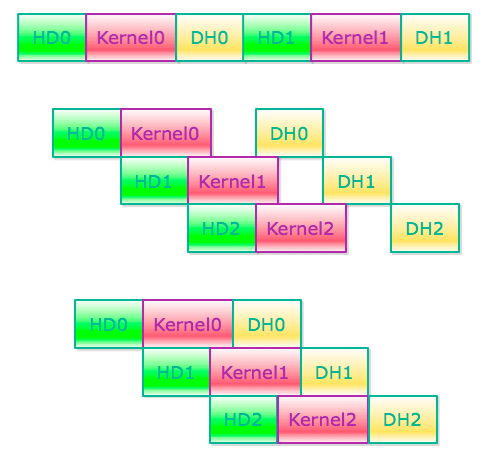
\includegraphics[width=120mm]{concurrent.png}
	\caption{Top: all operation in default stream. Mid: concurrent streams with one copy engine. Bottom: concurrent streams with two copy engine.}
	\label{concurrent}
\end{figure}

\section{Results}
Both CPU and GPU implementations was running on the TACC Stampede Supercomputer. The CPU is Intel® Xeon® E5-2680 2.7GHz Processors. And the GPU is NVIDIA K20 with 5120 MB GDDR5 memory and 2 copy engines. \par
The command line tool, nvprof, and the Nvidia Visual Profiler are used to profile the performance of our implementation. And the results are shown in the table below.

\section{Conclusion} 

\bibliographystyle{abbrv}
\begin{thebibliography}{9}
	\bibitem{Mark} 
Harries, M. (2012, December). How to Optimize Data Transfers in CUDA C/C++. Retrieved from https://devblogs.nvidia.com/parallelforall/how-optimize-data-transfers-cuda-cc/
	
\bibitem{Trade_off} 
Boyer, M. Choosing Between Pinned and Non-Pinned Memory. Retrieved from https://www.cs.virginia.edu/~mwb7w/cuda_support/pinned_tradeoff.html
	
\bibitem{Stream} 
Harries, M. (2012, December). How to Overlap Data Transfers in CUDA C/C++. Retrieved from https://devblogs.nvidia.com/parallelforall/how-overlap-data-transfers-cuda-cc/
	

\end{thebibliography}

\end{document}
